\section{Fallbeispiel 1 -- Lehrende und Betreuende}
    \label{section:findingsCaseStudy1}
    In diesem Fallbeispiel werden Übersichtsseiten
    über die Lehrenden und Betreuenden (Mitarbeiter) eines Studienportals
    der Fakultät \gls{ksw} der {\fernUni} klassifiziert.
    Anhand der Seite des Portals \gls{babw} wird dazu zunächst ein
    konzeptionelles Modell dieser Seiten sowie ein {\classificationModel} erstellt.
    Nach der einzelnen Klassifizierung dieser Seite folgt die separate Klassifizierung
    der Übersichtsseiten der Portale

    \begin{itemize}
        \item \gls{bapvs}\footnote{\url{http://www.fernuni-hagen.de/KSW/portale/bapvs/einstieg/lehrende-und-betreuende-im-b-a-pvs/}},
        \item \gls{bscpsy}\footnote{\url{http://www.fernuni-hagen.de/KSW/portale/bscpsy/einstieg/lehrende-und-betreuende-im-b-sc-psychologie/}} und
        \item \gls{mabm}\footnote{\url{http://www.fernuni-hagen.de/KSW/portale/mabm/einstieg/lehrende-und-betreuende-im-m-a-eeducation/}}.
    \end{itemize}

    Jede Klassifikation wird dabei in separaten Datenbanken gespeichert,
    um die Graphen isoliert betrachten zu können.
    Anschließend werden die Seiten aller Sites erneut klassifiziert und in
    einer gemeinsamen Datenbank gespeichert,
    um zu sehen, welchen Einfluss das auf die Graphen hat.
    Zu jeder Klassifikation werden einige Kennzahlen der Datenbank präsentiert.
    Anschließend erfolgt eine Betrachtung von Auffälligkeiten in den Klassifikationen und in den Annotationen.

    \subsection{Konzeptionelles Modell der Webseite}
    \label{section:findingsTeachersConceptualModel}
    Das konzeptionelle Modell wird in diesem Beispiel anhand
    der Übersichtsseite des Studienportals \gls{babw} beschrieben.
    Abbildung \ref{image:findingTeachersModelOverview} zeigt einen
    Ausschnitt dieser Seite, auf dem die wichtigsten Bereiche zu sehen sind.
    Eine Darstellung des Modells ist in Abbildung
    \ref{image:findingTeachersModelUml} zu sehen.

    \begin{figure}[htb]
        \centering
        
\includegraphics[width=\textwidth]{../resources/findings/case-study-1/model/overview.png}
        \caption{Die Webseite über Mitarbeiter des Portals \acrshort{babw}}
        \label{image:findingTeachersModelOverview}
    \end{figure}

    Die Webseite lässt sich in verschiedene Bereiche aufteilen.
    Zunächst einen Kopfbereich, der auf der linken Seite das Logo
    der {\fernUni} enthält.
    Dieses Bild ist gleichzeitig ein Link zur Hauptseite der Universität. 
    Auf der rechten Seite enthält der Kopfbereich einige Links zu den verschiedenen
    Bereichen der Site.
    Direkt unter dem Kopfbereich befindet sich der Name des Studienportals,
    welcher gleichzeitig ein Link auf die Einstiegsseite des Portals ist.
    Darunter befindet sich auf der linken Seite ein weiterer Navigationsbereich,
    der Verweise auf die Unterseiten des aktuellen Bereichs enthält.
    Rechts daneben findet sich zunächst der Titel der Seite,
    gefolgt von einem kurzen einleitenden Absatz.
    Alle bisher genannten Elemente der Seite finden sich in sehr ähnlicher Form
    auch auf anderen Seiten wieder.
    Die dem einleitenden Absatz folgende Liste aller Lehrenden und Betreuenden unterscheidet die Seite hingegen von anderen.
    Für jeden Mitarbeiter sind eine Reihe an Informationen dargestellt.
    Neben einem Bild ist das der Name des Lehrgebiets, in dem er tätig ist.
    Dieser Name ist außerdem ein Link auf eine Seite über dieses Gebiet.
    Es folgen der Name des Mitarbeiters
    und einige Kontaktinformationen.
    Dies können eine E-Mail-Adresse, eine Telefonnummer
    und bei einigen wenigen Kontakten auch eine Faxnummer und ein Raum sein.

    \begin{figure}[htb]
        \centering
        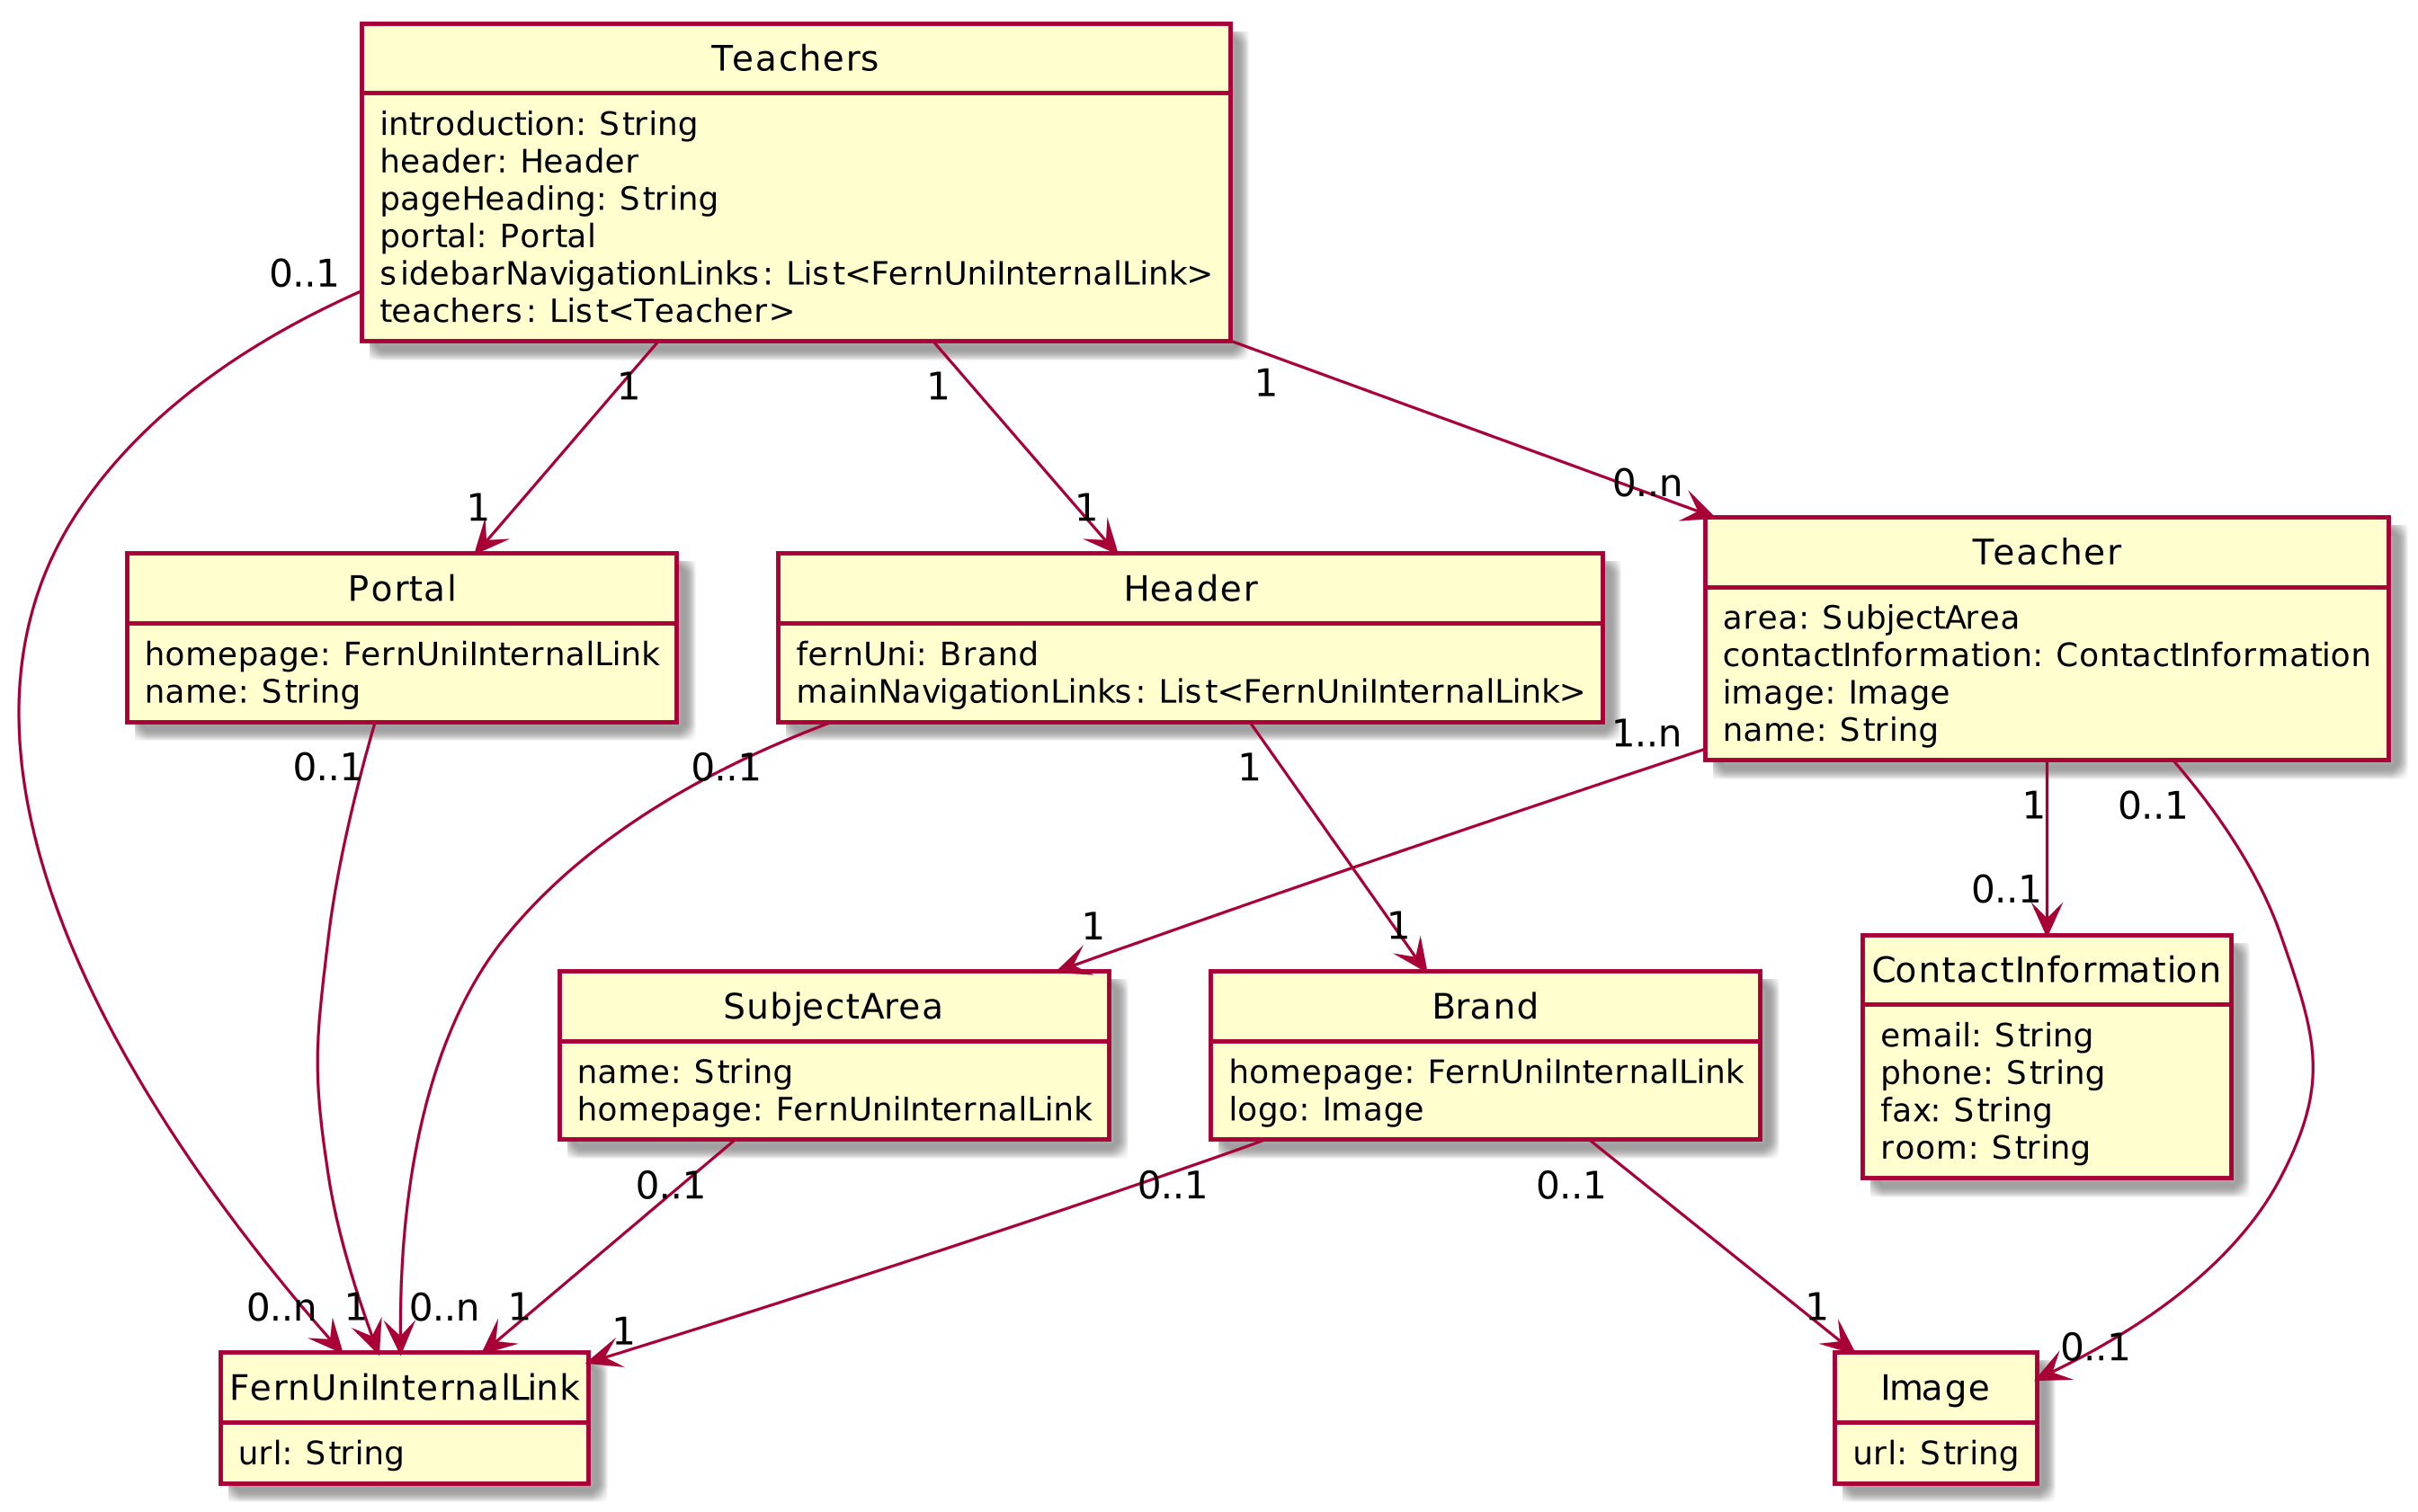
\includegraphics[scale=\imageScalingFactor]{../resources/findings/case-study-1/model/model.png}
        \caption{Das konzeptionelle Modell einer Webseite über Mitarbeiter}
        \label{image:findingTeachersModelUml}
    \end{figure}
    \subsection{Das {\classificationModel}}
    \label{section:findingsNewsClasses}
    Bei der Analyse der Nachrichtenseite wurde deutlich,
    dass einige Teile konzeptionell identisch mit denen aus dem ersten Beispiel sind.
    Die allgemeinen Klassendefinitionen aus Listing \ref{listing:findingsTeachersCommon}
    werden deshalb hier wiederverwendet.
    Die speziellen Definitionen für Nachrichtenseiten sind in
    Listing \ref{listing:findingsNewsSpecial}
    aufgeführt\footnote{Der Selektor in den Zeilen \ref{line:newsWctdInvalidSelectorStart}
    bis \ref{line:newsWctdInvalidSelectorEnd} wurde aus Gründen der Lesbarkeit umgebrochen,
    was syntaktisch nicht erlaubt ist.}.

    \lstinputlisting[
        label=listing:findingsNewsSpecial,
        caption=Das {\classificationModel} der Webseite \"uber aktuelle Meldungen,
        language=wccdl,
        inputencoding=utf8/latin1,
        style=wccdl,
        escapechar=|
    ]{../resources/findings/case-study-2/classification-model/NewsOverview.wctd}

    Die Seitenklasse \texttt{NewsOverview} enthält Features für die
    allgemeinen Bereiche der Seite sowie für die Referenzen auf die vorherige und die nächste
    Nachrichtenseite. Diese {\referenceFeature}s werden alle als \texttt{FernUniInternalLink} klassifiziert.
    Nicht zuletzt besitzt \texttt{NewsOverview} ein {\collectionFeature} für die Meldungen.
    Eine Nachricht wird durch die Klasse \texttt{News} repräsentiert,
    ihr Datum durch \texttt{NewsDate}, ihre Überschrift durch \texttt{NewsHeading}
    und ihre Absätze durch \texttt{NewsSection}.
    Die Überschrift enthält auch einen Link,
    der ebenfalls als \texttt{FernUniInternalLink} klassifiziert wird.
    Das Feature \texttt{sections} wurde auskommentiert.
    Der Grund ist, dass für die Absätze einer Nachricht kein Selektor ermittelt werden konnte,
    mit dem eine sinnvolle Klassifizierung möglich ist.
    Um dies zu erklären, ist eine Betrachtung der \gls{html}-Struktur der Nachrichtenliste notwendig.
    Diese Struktur ist in Listing \ref{listing:findingsNewsEvilHtmll}
    zu sehen, wobei konkrete textuelle Inhalte entfernt wurden,
    da sie für das Verständnis der Problematik irrelevant sind.

    \lstinputlisting[
        label=listing:findingsNewsEvilHtmll,
        caption=Die HTML-Repräsentation der Nachrichtenliste der Seiten über aktuelle Meldungen,
        style=html
    ]{../resources/findings/case-study-2/news.html}

    Aus diesem Fragment geht hervor,
    dass Nachrichten nicht in einzelne \gls{html}-Elemente gekapselt sind.
    Stattdessen befinden sich alle Elemente aller Nachrichten auf derselben Hierarchieebene.
    Nachrichten werden nur durch ein \texttt{hr}-Element voneinander getrennt,
    was sich das {\classificationModel} zunutze machen kann.
    Aufgrund der fehlenden Kapselung ist es aber mit den zur Verfügung
    stehenden CSS- und XPath-Selektoren nicht möglich festzustellen,
    welche Elemente als \texttt{NewsSection} zu klassifizieren sind.
    Der {\cssSelector} \texttt{p} würde bspw. alle Absätze aller Nachrichten selektieren.
    Erschwerend kommt hinzu, dass Absätze nicht nur \texttt{p},
    sondern auch andere Elemente sein können und dass jede Nachricht eine andere Anzahl an Absätzen besitzt.
    Informell ausgedrückt wäre ein Selektor notwendig,
    der ausgehend vom aktuellen Kontextelement (das \texttt{hr}-Element) alle Elemente
    ab dem ersten \texttt{h4}-Element bis zum nächsten \texttt{hr} selektiert.
    Das ist mit CSS nicht möglich, da es keine Selektoren für Geschwister des Kontextelementes gibt.
    XPath besitzt diese zwar, allerdings konnte auch mit diesen kein
    Ausdruck umgesetzt werden, der nur die Absätze der aktuellen Nachricht herausfiltert.
    Die einzige Lösung -- ohne das HTML anzupassen -- ist für jede Nachricht eine spezielle Klasse zu entwickeln.
    Durch eine solche 1:1-Beziehung kann jede Klasse individuelle und gleichzeitig
    eindeutige Selektoren für die Absätze enthalten.

    \subsection{Kennzahlen}
    Auch in diesem Fallbeispiel wurde eine Reihe an Kennzahlen ermittelt,
    die in diesem Kapitel präsentiert werden.

    \paragraph{Struktur eines Graphs}
    Zum Verständnis der Zahlen trägt Abbildung \ref{image:findingNewsFiguresDbModel} bei,
    welches den Aufbau des Graphs visualisiert.
    Wegen der beschriebenen Überschneidung mit dem ersten Fallbeispiel,
    sind die entsprechenden Knoten hier nicht nochmals dargestellt.
    Wie im vorherigen Beispiel wird außerdem auf die Darstellung von
    Referenzen verzichtet.

    \begin{figure}[htb]
        \centering
        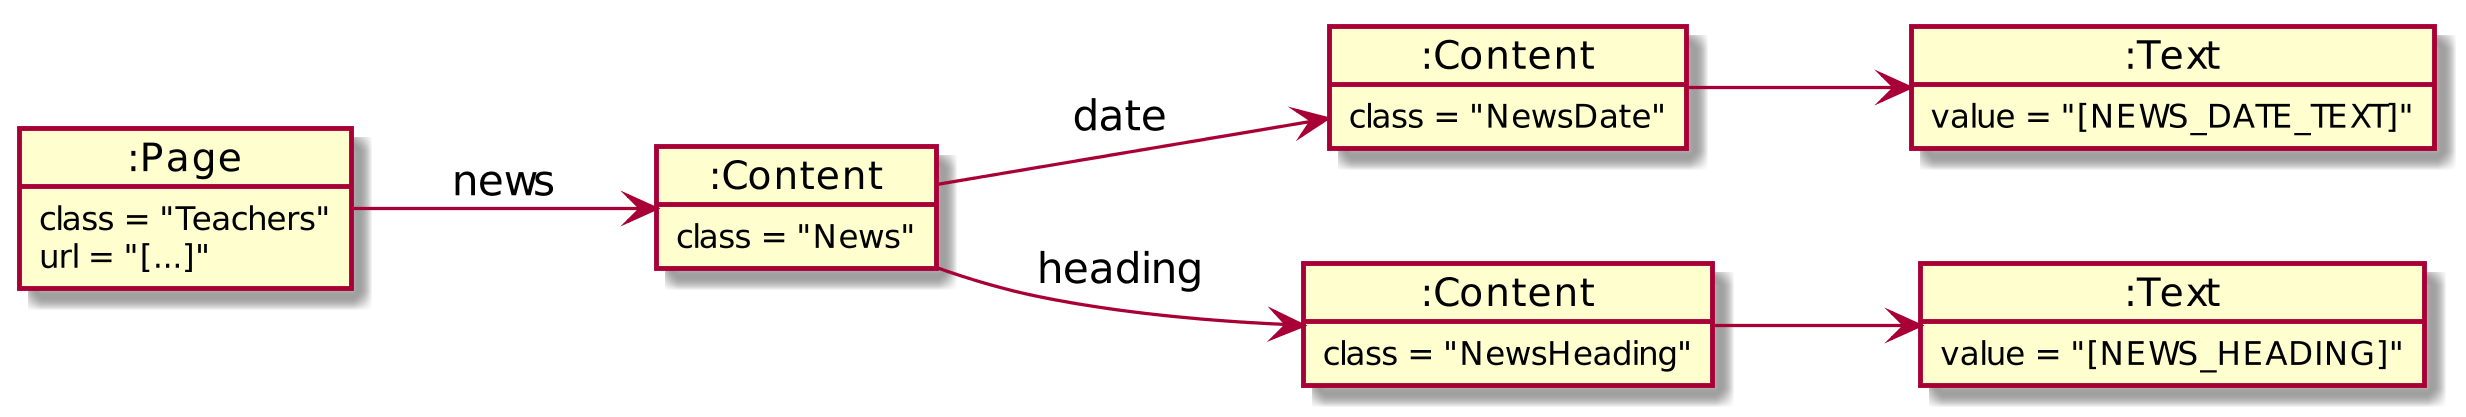
\includegraphics[scale=\imageScalingFactor]{../resources/findings/case-study-2/dbmodel.png}
        \caption{Struktur des Graphs einer Seite über aktuelle Meldungen}
        \label{image:findingNewsFiguresDbModel}
    \end{figure}

    \paragraph{Präsentation der Kennzahlen}
    Die folgenden Tabellen präsentieren die gesammelten Kennzahlen.
    Die Bedeutung einzelner Kennzahlen wurde bereits beim ersten Beispiel erläutert,
    die entsprechend auch hier gelten.
    Die Gruppierung der Knoten nach ihren Labels ist in Tabelle
    \ref{table:findingsNewsFiguresNodesByLabel} zu sehen.
    Die Häufigkeit der Inhaltsklassen stellt Tabelle
    \ref{table:findingsNewsFiguresContentNodesByClass} dar.
    Tabelle \ref{table:findingNewsFiguresEdgesByLabel} gruppiert die Kanten der Datenbank
    nach ihren Labels und Tabelle
    \ref{table:findingsNewsFiguresEdgesByStartEndNodeLabel}
    stellt heraus, welche Knotenarten diese Kanten verbinden.
    Zuletzt betrachtet Tabelle \ref{table:findingsNewsFiguresSharedNodes}
    die Frage, welche Knoten mehrfach referenziert wurden.

    \begin{table}[htb]
        \begin{subtable}[c]{0.3\textwidth}
            \centering
            \begin{tabular}{|l|c|}
                \hline
                \textbf{Label}  & \multicolumn{1}{l|}{\textbf{Anzahl}} \\ \hline
                Content         & 124                                  \\ \hline
                Page + Resource & 5                                    \\ \hline
                Resource        & 53                                   \\ \hline
                Site            & 1                                    \\ \hline
                Text            & 77                                   \\ \hline
                \hline
                \textbf{Summe}  & 260                                  \\ \hline
            \end{tabular}
            \subcaption{Knoten gruppiert nach Labels für Seiten über aktuelle Meldungen}
            \label{table:findingsNewsFiguresNodesByLabel}
        \end{subtable}
        \begin{subtable}[c]{0.3\textwidth}
            \centering
            \begin{tabular}{|l|c|}
                \hline
                \textbf{Klasse} & \multicolumn{1}{l|}{\textbf{Anzahl}} \\ \hline
                Brand           & 1                                    \\ \hline
                Header          & 1                                    \\ \hline
                News            & 41                                   \\ \hline
                NewsDate        & 38                                   \\ \hline
                NewsHeading     & 41                                   \\ \hline
                PageHeading     & 1                                    \\ \hline
                Portal          & 1                                    \\ \hline
                \hline
                \textbf{Summe}  & 260                                  \\ \hline
            \end{tabular}
            \subcaption{\texttt{Content}-Knoten gruppiert nach ihrer Klasse für Seiten über aktuelle Meldungen}
            \label{table:findingsNewsFiguresContentNodesByClass}
        \end{subtable}
        \begin{subtable}[c]{0.3\textwidth}
            \centering
            \begin{tabular}{|l|c|}
                \hline
                \textbf{Label} & \multicolumn{1}{l|}{\textbf{Anzahl}} \\ \hline
                Reads          & 80                                   \\ \hline
                References     & 87                                   \\ \hline
                Owns           & 145                                  \\ \hline
                \hline
                \textbf{Summe} & 312                                  \\ \hline
                \end{tabular}
            \subcaption{Kanten gruppiert nach Labels für Seiten über aktuelle Meldungen}
            \label{table:findingNewsFiguresEdgesByLabel}
        \end{subtable}

        \begin{subtable}[c]{0.5\textwidth}
            \centering
            \begin{tabular}{|l|c|}
                \hline
                \textbf{Start $\rightarrow$ Ziel} & \multicolumn{1}{l|}{\textbf{Anzahl}} \\ \hline
                (:Content) $\rightarrow$ (:Content)     & 83                                   \\ \hline
                (:Content) $\rightarrow$ (:Resource)    & 49                                   \\ \hline
                (:Page) $\rightarrow$ (:Content)        & 57                                   \\ \hline
                (:Page) $\rightarrow$ (:Page)           & 13                                   \\ \hline
                (:Page) $\rightarrow$ (:Resource)       & 25                                   \\ \hline
                (:Site) $\rightarrow$ (:Page)           & 5                                    \\ \hline
                \textbf{Summe}                    & 232                                  \\ \hline
            \end{tabular}
            \subcaption{Kanten gruppiert nach Labels der Start- und Zielknoten für Seiten über aktuelle Meldungen}
            \label{table:findingsNewsFiguresEdgesByStartEndNodeLabel}
        \end{subtable}
        \begin{subtable}[c]{0.5\textwidth}
            \centering
            \begin{tabular}{|l|c|}
                \hline
                \textbf{Knoten} & \multicolumn{1}{l|}{\textbf{Anzahl}} \\ \hline
                PageHeading     & 1                                    \\ \hline
                Portal          & 1                                    \\ \hline
                Header          & 1                                    \\ \hline
                News            & 1                                    \\ \hline
                NewsDate        & 1                                    \\ \hline
                Seiten          & 4                                    \\ \hline
                Unterseiten     & 5                                    \\ \hline
                :Text           & 2                                    \\ \hline
                \textbf{Summe}  & 16                                   \\ \hline
                \end{tabular}
            \subcaption{Knoten mit mehreren eingehenden Kanten für Seiten über aktuelle Meldungen}
            \label{table:findingsNewsFiguresSharedNodes}
        \end{subtable}
        \label{table:findingsNewsFigures}
        \caption{Kennzahlen der Seiten über aktuelle Meldungen}
    \end{table}
    \subsection{Annotationen}
    \subsection{Unregelmäßigkeiten in der Klassifikation des Portals \acrshort{babw}}
    \label{section:findingsTeachersAbnormalitiesBabw}
    Dieses Kapitel stellt die Auffälligkeiten in der Klassifikation
    der Seite der Lehrenden und Betreuenden im Studienportal
    \gls{babw} vor.
    Zusätzlich erfolgt eine Erklärung,
    wodurch die jeweilige Unregelmäßigkeit begründet ist.

    \paragraph{Zwei Mitarbeiter ohne Lehrgebiet}
    Die Klassifikation enthält für zwei Mitarbeiter kein Lehrgebiet.
    Im ersten Fall nennt die Webseite kein Lehrgebiet,
    weshalb die Klassifikation an dieser Stelle korrekt ist.
    Der zweite Kontakt ist ein Mitarbeiter einer fremden Universität,
    weshalb dessen Lehrgebiet kein Verweis auf eine andere Seite,
    sondern einfacher Text ist.
    Der verwendete Selektor \texttt{div.team-member-des > p > a:first-child}
    hat diesen Text nicht erfasst, da er einen Link sucht.

    \paragraph{Unvollständige Namen zweier Mitarbeiter}
    Zwei Kontakte besitzen laut Klassifikation den Namen "`Prof."' bzw. "`Dr."'.
    In diesen Fällen stehen Titel und Name in getrennten \texttt{strong}-Elementen.
    Da der Name eines Mitarbeiters ein skalares Feature ist,
    wurde nur das erste Element vom System erfasst.

    \paragraph{Falsche und fehlende Hervorhebungen durch Annotationen}
    Einige Elemente der Seite wurden durch Annotator inkorrekt oder nicht hervorgehoben.
    Aus Abbildung \ref{image:findingTeachersAnnotationsOverview} geht bereits hervor,
    dass Bilder davon betroffen sind.
    Abbildung \ref{image:findingTeachersBaBwWrongAnnotations}
    veranschaulicht, dass Telefonnummern und Raumangaben oftmals verschoben annotiert werden.
    Der Grund ist der
    beschriebene Konflikt bei der Bestimmung eines eindeutigen
    Selektors\footnote{vgl. Kapitel \ref{section:solutionDetailsClassificationServiceClassification}}.
    Außerdem fällt auf, dass die E-Mail-Adresse trotz korrekter Klassifizierung
    überhaupt nicht markiert wurde.

    \begin{figure}[htb]
        \centering
        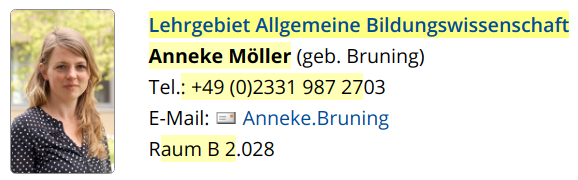
\includegraphics[scale=\screenshotScaleFactor]{../resources/findings/case-study-1/babw/annotations/missing-annotation.png}
        \caption{Ein Beispiel fehlerhafter Annotationen im Portal \acrshort{babw}}
        \label{image:findingTeachersBaBwWrongAnnotations}
    \end{figure}

    \subsection{Unregelmäßigkeiten in der Klassifikation des Portals \acrshort{bapvs}}
    \label{section:findingsTeachersAbnormalitiesBaPVS}
    Die Klassifikation des Lehrgebietes \gls{bapvs}
    weist ebenfalls einige Unregelmäßigkeiten auf,
    die dieses Kapitel beschreibt.

    \paragraph*{Doppelt klassifizierte Mitarbeiter}
    Drei Mitarbeiter des Portals wurden doppelt klassifiziert.
    Der Grund ist eine abweichende HTML-Repräsentation bei diesen Mitarbeitern,
    die in Listing \ref{listing:findingsTeachersBaPVSHtmlSource} zu sehen ist.

    \lstinputlisting[
        label=listing:findingsTeachersBaPVSHtmlSource,
        caption=Eine abweichende HTML-Struktur eines Mitarbeiters des Portals BaPVS,
        style=html
    ]{../resources/findings/case-study-1/bapvs/teacher.html}

    Im Vergleich zur erwarteten Struktur wiederholt sich
    das \texttt{div}-Element mit der Klasse \texttt{grid},
    weshalb der verwendete Selektor \texttt{section\#content div.grid}
    betroffene Mitarbeiter doppelt erfasst.
    Bei der zweiten Klassifizierung
    (beim inneren \texttt{div}-Element) kann das System kein Bild finden,
    weshalb sie von der Ersten abweicht und ein zweiter \texttt{Teacher}-Knoten angelegt wird.
    Diese teilen sich aber die restlichen Informationen,
    also Name, Lehrgebiet und Kontaktinformationen.
    Der dritte betroffene Mitarbeiter besitzt kein Bild,
    weshalb der \texttt{Teacher}-Knoten vollständig wiederverwendet werden kann.

    \paragraph*{Mitarbeiter ohne Lehrgebiet}
    Das Lehrgebiet eines einzelnen Mitarbeiters wurde vom System nicht erfasst.
    Anders als beim Portal \gls{babw} ist der Grund allerdings,
    dass vor dem Lehrgebiet der Text "`Auskunft erteilt auch:"' platziert ist.
    Der Selektor \texttt{div.team-member-des > p > a:first-child} findet
    das Lehrgebiet nicht, weil er nach einem \texttt{a}-Element sucht,
    welches das erste Kindelement seines Vaterelementes ist.
    Eine naheliegende Lösung ist die Änderung des Selektors,
    sodass er mit \texttt{a:first-of-type} endet.
    Bei der Erstellung des {\classificationModel}s,
    was auf Basis des Portals \gls{babw} geschah,
    wurde sich allerdings bewusst gegen diese Variante entschieden.
    Bei dem Mitarbeiter im \gls{babw}, für den kein Lehrgebiet erfasst
    wurde,
    hätte dieser Selektor nämlich dazu geführt,
    dass seine E-Mail-Adresse als Lehrgebiet erkannt wird.

    \paragraph*{Falscher Text als Name klassifiziert}
    Der Name eines Mitarbeiters ist laut Klassifikation
    "`Auskunft erteilt auch:"'.
    Der Grund ist, dass dieser Text in einem \texttt{strong}-Element steht,
    welches vor dem Namen auftaucht.
    Das System hat in diesem Fall erwartungskonform nur den ersten
    Treffer für das skalare Feature klassifiziert.
        
    \paragraph*{28 Mitarbeiter ohne Telefonnummer}
    Einige Kontakte besitzen in der Klassifikation keine Telefonnummer.
    Bei neun ist auch auf der Webseite keine zu finden.
    Bei den Restlichen ist der Nummer nicht "`Tel.: "'
    sondern "`Telefon: "' oder "`Tel:"' vorangestellt.
    Der Selektor hat die Telefonnummern deshalb nicht erkannt.
    
    \paragraph*{56 Mitarbeiter ohne Namen}
    Des Weiteren wurde für eine Vielzahl der Mitarbeiter kein Name erkannt,
    da sie weder in einem \texttt{strong}- noch einem \texttt{b}-Element stehen.
    Stattdessen befinden sie sich wie die Telefonnummer als reiner Text im \texttt{p}-Element
    oder in einem \texttt{a}-Element.

    \paragraph*{Inkorrekte Telefonnummern}
    Die Klassifikation enthält einige Telefonnummern,
    die neben der eigentlichen Nummer auch weitere Informationen enthalten.
    Ein Beispiel ist "`02331/987-4315 email: Lisa.Schaefer Sprechstunde: nach Vereinbarung via e-mail"'.
    Die Telefonnummer wird über einen {\xpathSelector} erfasst,
    der auf dem Seitenquelltext ausgeführt wird.
    Anders als beim Portal \gls{babw} existieren im Portal \gls{bapvs} Mitarbeiter,
    bei denen die Telefonnummer weder die letzte Angabe ist
    noch durch einen Zeilenumbruch im Quelltext beendet wird.
    Der Selektor der Telefonnummer erkennt sie deshalb
    nicht.

    \paragraph*{Unterschiede im konzeptionellen Modell der Seite}
    Im Vergleich zur klassifizierten Seite des Portals \gls{babw}
    sind auch zwei Unterschiede im konzeptionellen Modell der Seite deutlich geworden.
    Der Name eines Mitarbeiters ist in einigen Fällen
    auch ein Link auf eine Detailseite.
    Außerdem besitzen einige Mitarbeiter Sprechzeiten.

    \paragraph*{Falsch annotierte Telefonnummern}
    Bei der Betrachtung der Annotationen des Portals \gls{babw}
    ist bereits aufgefallen, dass sie für Telefonnummern
    mehrmals verschoben sind.
    Dies ist im Fall des Portals \gls{bapvs} ebenfalls zu beobachten,
    allerdings in einem deutlicheren Ausmaß,
    wie Abbildung \ref{image:findingTeachersBaPVSWrongPhone} zeigt.

    \begin{figure}[htb]
        \centering
        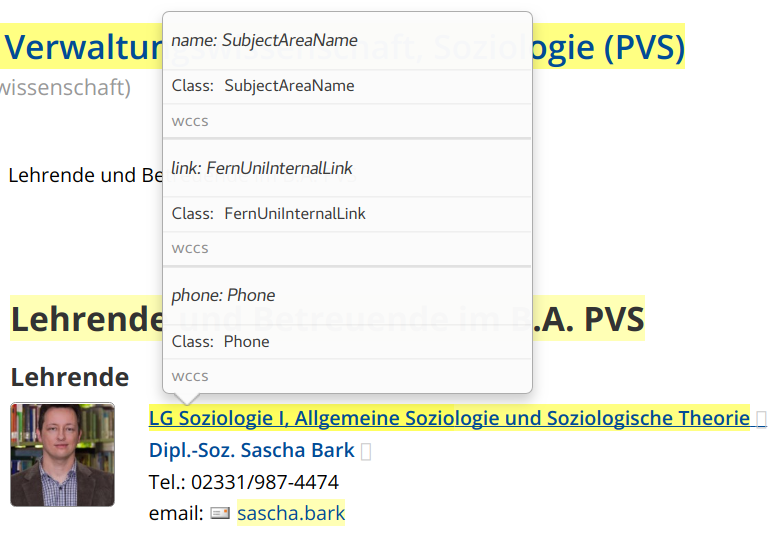
\includegraphics[scale=\screenshotScaleFactor]{../resources/findings/case-study-1/bapvs/annotations/triple-annotation.png}
        \caption{Ein Beispiel verschobener Annotation im Portal \acrshort{bapvs}}
        \label{image:findingTeachersBaPVSWrongPhone}
    \end{figure}

    Bei der Bestimmung des eindeutigen Selektors,
    wird die Position des klassifizierten Textes in der Eigenschaft
    \texttt{innerText} gesucht und als Versatz im Startelement
    verwendet\footnote{vgl. Kapitel \ref{section:solutionDetailsClassificationServiceClassification}}.
    In den betroffenen Fällen befindet sich zwischen der Telefonnummer
    und der E-Mail-Adresse nur ein \texttt{br}-Element,
    aber kein physischer Zeilenumbruch im
    Seitenquelltext\footnote{vgl. Listing \ref{listing:findingsTeachersHtmlSource}}.
    Die Telefonnummer, die über einen {\xpathSelector} ermittelt wird,
    enthält deshalb zu viele Informationen (siehe oben).
    Das \texttt{br}-Element wird über die verwendete Methode \texttt{document.evaluate} nicht zu einem Zeilenumbruch übersetzt.
    Die einzelnen Angaben in der Telefonnummer sind stattdessen nur durch ein Leerzeichen getrennt.
    In \texttt{innerText} wird das \texttt{br}-Element aber zu einem Umbruch,
    weshalb der klassifizierte Text in dieser Eigenschaft nicht gefunden wird.
    Als Versatz wird deshalb $-1$ gespeichert.
    Annotator setzt die Annotation deshalb an den Anfang des umschließenden Elementes.

    \subsection{Unregelmäßigkeiten in der Klassifikation des Portals "`\acrshort{bscpsy}"'}
    Auch bei der Klassifizierung des Portals \gls{bscpsy}
    sind im Vergleich zu den vorherigen Beobachtungen zwei neue
    Auffälligkeiten aufgetreten.

    \paragraph{Leere Einleitung}
        Die Klassifikation enthält eine Einleitung.
        Allerdings besteht diese nur aus einem Leerzeichen,
        da die Webseite einen Absatz besitzt,
        auf den der Selektor zutrifft.
        Dieser enthält aber nur das Zeichen \texttt{\&nbsp;}.

    \paragraph{Zwei Mitarbeiter ohne E-Mail-Adresse}
        Des Weiteren wurden zwei Mitarbeiter ohne E-Mail-Adresse klassifiziert.
        Bei einem ist dies korrekt, da die Webseite ebenfalls keine Adresse enthält.
        Im anderen Fall wurde sie nicht erkannt,
        da die \gls{uri} kein vorangestelltes \texttt{mailto:} enthält
        und deshalb nicht vom Selektor erfasst wurde.
        
    \subsection{Unregelmäßigkeiten in der Klassifikation des Portals "`MaBm"'}
    Nicht zuletzt enthält auch die Klassifikation des Portals
    "`M.A. Bildung und Medien: eEducation"'
    zwei Auffälligkeiten,
    die hier kurz aufgezeigt werden.

    \paragraph{Zwei Lehrende ohne Lehrgebiet}
    Im Falle zweier Mitarbeiter wurde kein Lehrgebiet erkannt.
    Der Grund ist eine erneute andere Struktur des \glspl{html}.
    In diesen Fällen ist der Link auf das Lehrgebiet
    in ein strong Element eingebettet, weshalb es nicht erkannt wurde.

    \paragraph{Inkorrekte Nabem zweier Mitarbeiter}
    Bei den gleichen Mitarbeitern enthält ihr Name außerdem ihr Lehrgebiet.
    Wie beschrieben enthält das strong Element das Lehrgebiet,
    aber auch den Namen des Mitarbeiters.
    Der Selektor des Namens des Mitarbeiters erfasst genau dieses strong Element.

